% We switch to portrait mode. This works as advertised.
\documentclass[a0,portrait]{a0poster}
% You might find the 'draft' option to a0 poster useful if you have
% lots of graphics, because they can take some time to process and
% display. (\documentclass[a0,draft]{a0poster})

\usepackage[margin=40mm]{geometry}

%\usepackage[utf8]{inputenc}

% Switch off page numbers on a poster, obviously, and section numbers too.
\pagestyle{empty}
\setcounter{secnumdepth}{0}

%fonts
\usepackage[T1]{fontenc}
\usepackage{kpfonts}
%\usepackage{roboto}
\usepackage{fontspec}
%\usepackage[oldstylenums, largesmallcaps]{kpfonts}
%\setmainfont[Numbers=OldStyle]{Tex Gyre Pagella}
\setmainfont{Tex Gyre Pagella}
\setsansfont[BoldFont=infini_bold,ItalicFont=infini_ital]{infini_romain}
%\setsansfont[BoldFont=Lovelo-LineBold]{Lovelo-LineBold}
%\setsansfont{Choplin-Medium-DEMO}
%\setsansfont{RobotoSlab-Bold}
%\setsansfont[StylisticSet=4]{MEgalopolisExtra}
%\renewcommand*\sfdefault{ugq}

\usepackage{hyperref}
\hypersetup{%
	pdftitle={Importance of many-body correlations in glass transition: an example from polydisperse hard spheres},%the title
	pdfauthor={Mathieu Leocmach},%your name
	hidelinks=true,
}

%proper math and math symbols
%\usepackage{amsmath}
\usepackage{amssymb}

\usepackage{siunitx}

\usepackage{tabu}
\usepackage{multirow}

% Allow the usage of graphics (.jpg, .png, etc.) in the document
\usepackage{graphicx}
\usepackage{tikz}
\usetikzlibrary{arrows,shapes,backgrounds, positioning, intersections, decorations.markings, decorations.shapes, mindmap, shapes.geometric, matrix, patterns}

\usepackage{pgfplots}
\pgfplotsset{compat=1.9}
\usepackage{pgfplotstable}
%\usepgfplotslibrary{units}
\usepgfplotslibrary{groupplots}
\pgfplotsset{every axis/.append style={xlabel near ticks,ylabel near ticks,mark size={0.2em}}}
\pgfplotsset{every axis plot post/.append style={very thick}}

\usepgfplotslibrary{external}
%\tikzexternalize
\tikzsetexternalprefix{fig_poster_palavas/}
\tikzset{external/system call={lualatex \tikzexternalcheckshellescape -halt-on-error -interaction=batchmode -jobname "\image" "\texsource"}}


\usepackage{ragged2e}
\RaggedRight

\usepackage{framed}
\colorlet{shadecolor}{lightgray!50!white}

\definecolor{Main}{rgb}{1, 0.57, 0}
\definecolor{Accent1}{rgb}{1,0.28,0}
\definecolor{Accent2}{rgb}{1,0.74,0}

% see documentation for a0poster class for the size options here
\let\Textsize\normalsize
\def\Norulehead#1{\noindent\hbox to \hsize{\hfil\LARGE\textcolor{Main}{\textsf{#1}}}\bigskip}
\def\Head#1{\Norulehead{#1\hrulefill}}
\def\LHead#1{{\LARGE #1}\smallskip}
\def\Subhead#1{\noindent{\large\color{Accent1}\textsc{#1}}}
\def\Title#1{\noindent{\VeryHuge\color{Accent2}\raggedright\textsf{
\addfontfeature{Ligatures=Rare}{#1}}}}

\renewcommand{\descriptionlabel}[1]{\hspace{\labelsep}\textcolor{Accent2}{\textsc{#1}}}

% The textpos package is necessary to position textblocks at arbitary 
% places on the page.
\usepackage[absolute,overlay,showboxes
]{textpos}
% Set up the grid
%
% Note that [40mm,40mm] is the margin round the edge of the page --
% it is _not_ the grid size. That is always defined as 
% PAGE_WIDTH/HGRID and PAGE_HEIGHT/VGRID. In this case we use
% 15 x 25. This gives us a wide central column for text (7 grid
% spacings) and two narrow columns (3 each) at each side for 
% pictures, separated by 1 grid spacing.
%
% Note however that texblocks can be positioned fractionally as well,
% so really any convenient grid size can be used.
%
\TPGrid[40mm,40mm]{15}{25}  % 3 - 1 - 7 - 1 - 3 Columns

% Mess with these as you like
\parindent=0pt
%\parindent=1cm
\parskip=0.5\baselineskip

\usepackage{paralist}

%bibliography
\usepackage{natbib}
\usepackage{bibentry}
\def\newblock{\hskip .11em plus .33em minus .07em}



\newlength{\mylength}

%\includeonly{}

\begin{document}
\pgfplotscreateplotcyclelist{earthy}{%
red!40!black,
red!60!black,
red!80!black,
red,
red!80!yellow,
red!60!yellow,
red!40!yellow,
}

\bibliographystyle{notitle}
%\nobibliography{sift}

% Understanding textblocks is the key to being able to do a poster in
% LaTeX. In
%
%    \begin{textblock}{wid}(x,y)
%    ...
%    \end{textblock}
%
% the first argument gives the block width in units of the grid
% cells specified above in \TPGrid; the second gives the (x,y)
% position on the grid, with the y axis pointing down.

% You will have to do a lot of previewing to get everything in the 
% right place.

% This gives good title positioning for a portrait poster.
% Watch out for hyphenation in titles - LaTeX will do it
% but it looks awful.


\begin{center}
\Title{
IMPORTANCE of MANY-BODY CORRELATIONS in GLASS TRANSITION: {\Huge an example from polydisperse hard spheres}
}
\end{center}

\vfill
\LHead{Mathieu Leocmach,\hfill \textsc{Laboratoire de Physique, Ecole Normale Supérieure de Lyon}
}\hfill\texttt{\color{Accent1}mathieu.leocmach@polytechnique.org}

\LHead{John Russo \& Hajime Tanaka\qquad
\textsc{Institute of Industrial Science, the University of Tokyo}
%\hfill\raisebox{0pt}[0pt]{
%	\includegraphics[height=2\baselineskip,clip=true, trim=6mm 14mm 6mm 0]{NEW-Logo-ERC-OUTLINE}\;
%	\includegraphics[height=2\baselineskip]{logo_ums_grand}\;
%	\includegraphics[height=2\baselineskip]{CNRSfilaire-Q}\;
%	\includegraphics[height=2\baselineskip]{CRPP}\;
%	\includegraphics[height=2\baselineskip]{logo_ens-lyon}
%}
}\\



\vfill
\begin{minipage}[t][3\TPVertModule]{6\TPHorizModule}
	\Head{Structure behind dynamic heterogeneities?}
	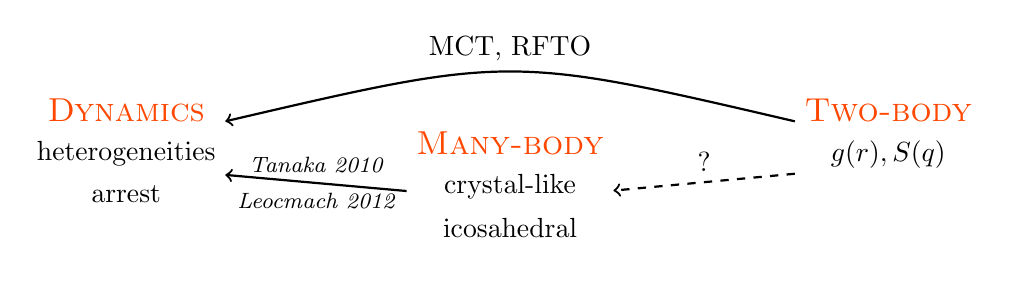
\begin{tikzpicture}
		\begin{scope}[every node/.style={rectangle split},every text node part/.style={font=\large\sffamily\scshape,Accent1}]
			\node (dyn) {Dynamics\nodepart{two}heterogeneities\nodepart{three}arrest};
			\node[anchor=base east] (twobody) at ($(dyn.base west) + (\textwidth,0)$) {Two-body\nodepart{two}$g(r), S(q)$};
			\node[anchor=north] (struct) at ($(dyn.base east)!0.5!(twobody.base west)$){Many-body\nodepart{two} crystal-like\nodepart{three}icosahedral};
		\end{scope}
		
		\draw[->, dashed, thick] (twobody) -- (struct) node[midway, above] {?};
		\draw[->, thick] (struct) -- (dyn)  node[midway, above, font=\footnotesize\itshape] {Tanaka 2010} node[midway, below, font=\footnotesize\itshape] {Leocmach 2012};
		\draw[->, thick] (twobody.base west) ..controls ($(struct.north)+(0,2\baselineskip)$) .. (dyn.base east)  node[midway, above] {MCT, RFTO}; 
	\end{tikzpicture}
	Monte Carlo simulations, N=4000, polydisperse hard spheres
\end{minipage}
\hfill
\begin{minipage}[t][3\TPVertModule]{3\TPHorizModule}
	\Head{State points}
\begin{tikzpicture}
	\begin{axis}[%
		width=\columnwidth-2em,
		height=2\TPVertModule,
		xlabel={$\phi$},
		ylabel={$\beta p\sigma^3$},
		xmin=0.45, xmax=0.59, xtick={0.46, 0.49, ..., 0.59},
		ytick={9,11,...,27},
		]
		\addplot+[Accent1,every mark/.append style={fill=Accent1}] file{figures/fig1/circles.dat} node[pos=0, right=1em] {$\Delta=7\%$};
		\addplot+[Accent2, every mark/.append style={scale=0.8}, mark=square
] file{figures/fig1/squares.dat} node[pos=0, left] {$\Delta\nearrow 15\%$};
		\addplot[mark=diamond] coordinates {(0.5347,17) (0.5358, 17) (0.537528, 17)} node[pos=0, left] {$\Delta\searrow 0\%$};;
		%\addplot[domain=0.45:0.59, dashed] {(1+x+x^2-x^3)/(1-x)^3};
	\end{axis}
	\end{tikzpicture}
\end{minipage}
\hfill
\colorbox{lightgray}{\begin{minipage}[t][3\TPVertModule]{3\TPHorizModule}
	\Head{Take home}

\end{minipage}}

\vfill
\begin{minipage}[t][3.5\TPVertModule]{5.4\TPHorizModule}
	\Head{Two-body order parameters}
	\Subhead{Two-body excess entropy}
	\[
		s_2(i) = -\frac{\rho k_B}{2}\sum_j \left[g(r_{ij})\log(g(r_{ij}))-g(r_{ij})+1\right]
	\]
	
	\vfill
	\Subhead{Pair free energy}
	\[
		f_2=\sum_i f_2(i)=-k_BT\sum_i \log(v(i)/\lambda),
	\]
	Free volume $v(i)$ by shifting the faces of the Voronoi polyhedron by $\sigma(i)/2$. 
	$\lambda$ is the thermal de Broglie wavelength. \textit{\footnotesize Aste \& Coniglio, EPL (2004)}
\end{minipage}
\hfill
\begin{minipage}[t][3.5\TPVertModule]{9.25\TPHorizModule}
	\Head{Many-body order parameters}
	Steinhardt (1984) bond orientational order from spherical harmonics $Y_{\ell m}$:\hfill
$\displaystyle q_{\ell m}(i)=\frac{1}{N_b(i)}\sum_{j=1}^{N_b(i)} Y_{\ell m}(\mathbf{\hat{r}_{ij}})$
	
	\vfill
	\Subhead{6-fold symmetry} \hfill $\displaystyle q_6 = \sqrt{\frac{4\pi}{13} \sum_{m=-6}^{6} |q_{6 m}|^2 }$ \hfill 
	\Subhead{Icosahedral symmetry} \hfill $\displaystyle w_6 = \sum_{m_1+m_2+m_3=0} 
			\left( \begin{array}{ccc}
				6 & 6 & 6 \\
				m_1 & m_2 & m_3 
			\end{array} \right)
			q_{6 m_1} q_{6 m_2} q_{6 m_3}$

	\vfill
	\Subhead{6-fold symmetry of the second shell} \hfill $q_{6m}\xrightarrow{\text{coarse-grain}} Q_{6m}  \rightarrow Q_6(i)$. \textit{\footnotesize Lechner \& Dellago J. Chem. Phys. (2008)}

	\vfill
	\Subhead{Crystallinity} \hfill $\displaystyle \text{C}(i)=\sum_{j=0}^{N_b(i)}\frac{\mathbf{q}_6(i)\cdot\mathbf{q}_6(j)}{|\mathbf{q}_6(i)|\,|\mathbf{q}_6(j)|}.$ \hfill $Q_6$ and C are specifically sensitive to crystal-like order.
\end{minipage}

\vfill
%\begin{minipage}[t][12.5\TPVertModule]{15\TPHorizModule}
	\hfill\begin{tikzpicture}
		\begin{groupplot}[%
		group style={
			group name=dis,
			group size=6 by 1,
			horizontal sep=0.02\textwidth,
			vertical sep = 4em,
			y descriptions at=edge left,
			},%
		width=0.14\columnwidth,%
		height=8\baselineskip,%
		scale only axis,
		axis on top,
		ymax=2,
		ymin=0,
		extra y ticks={1}, extra y tick labels={}, extra tick style={grid=major},%
		no markers,%
		every axis plot post/.append style={Accent1, thick},
		ylabel={Mobility},
		ylabel absolute, every axis y label/.append style={anchor=base, yshift=1.5em},
		every axis title/.style={anchor=base east, at={(1,1)},yshift=\baselineskip, inner xsep=0},
		]
		\nextgroupplot[xlabel=$s_2$, xmin=-70,xmax=0,xtick={-70,-50,...,0}, title=\Subhead{Two-body excess entropy}]
		\addplot table[x index=0, y index=2]{s2_distrib_mobility.txt};
		
		\nextgroupplot[xlabel=$f_2$, xmin=0,xmax=25,xtick={0,5,...,20}, title=\Subhead{Pair free energy}]
		\addplot table[x index=0, y index=2]{f2_distrib_mobility.txt};
		
		\nextgroupplot[xlabel=$q_6$, xmin=0,xmax=0.8,xtick={0,0.2,...,0.8}, title=\Subhead{6-fold symmetry}]
		\addplot table[x index=0, y index=2]{q6_distrib_mobility.txt};
		
		\nextgroupplot[xlabel=$100w_6$, xmin=-5.2,xmax=1, title=\Subhead{Icosahedral symmetry}]
		\addplot table[x expr=\thisrowno{0}*100, y index=2]{w6_distrib_mobility.txt};
		
		\nextgroupplot[xlabel=$Q_6$, xmin=0,xmax=0.6, title=\Subhead{Second shell 6-fold}]
		\addplot table[x index=0, y index=2]{Q6_distrib_mobility.txt};
		
		\nextgroupplot[xlabel=$C$, xmin=-6,xmax=12, xtick={-5,0,5,10}, title=\Subhead{Crystallinity}]
		\addplot table[x index=0, y index=2]{C_distrib_mobility.txt};
	\end{groupplot}
	\end{tikzpicture}

	\hfill\begin{tikzpicture}
		\begin{groupplot}[%
		group style={
			group name=dis,
			group size=6 by 1,
			horizontal sep=0.02\textwidth,
			vertical sep = 4em,
			y descriptions at=edge left,
			},%
		width=0.14\columnwidth,%
		height=8\baselineskip,%
		scale only axis,
		axis on top,
		ymode=log,%
		ymax=2e-1,
		ymin=1e-6,
		no markers,%
		every axis plot post/.append style={Accent1, thick},
		ylabel={Probability},
		ylabel absolute, every axis y label/.append style={anchor=base, yshift=1.5em},
		]
		\nextgroupplot[xlabel=$s_2$, xmin=-70,xmax=0,xtick={-70,-50,...,0}]
		\fill[gray!20] (axis cs:-70,1) rectangle (axis cs:-29.34,1e-7) node (s2) {};
		\addplot file{s2_distrib_mobility.txt};
		
		\nextgroupplot[xlabel=$f_2$, xmin=0,xmax=25,xtick={0,5,...,20}]
		\fill[gray!20] (axis cs:11.98,1e-7) rectangle (axis cs:25,1);
		\addplot file{f2_distrib_mobility.txt};
		
		\nextgroupplot[xlabel=$q_6$, xmin=0,xmax=0.8,xtick={0,0.2,...,0.8}]
		\fill[gray!20] (axis cs:0.495,1e-7) rectangle (axis cs:0.8,1);
		\addplot file{q6_distrib_mobility.txt};
		
		\nextgroupplot[xlabel=$100w_6$, xmin=-5.2,xmax=1]
		\fill[gray!20] (axis cs:-5.2,1e-7) rectangle (axis cs:-1.44,1);
		\addplot table[x expr=\thisrowno{0}*100]{w6_distrib_mobility.txt};
		
		\nextgroupplot[xlabel=$Q_6$, xmin=0,xmax=0.6]
		\fill[gray!20] (axis cs:0.234,1e-7) rectangle (axis cs:0.6,1);
		\addplot file{Q6_distrib_mobility.txt};
		
		\nextgroupplot[xlabel=$C$, xmin=-6,xmax=12, xtick={-5,0,5,10}]
		\fill[gray!20] (axis cs:5.11,1e-7) rectangle (axis cs:12,1);
		\addplot file{C_distrib_mobility.txt};
	\end{groupplot}
	\end{tikzpicture}

\Head{Spatial correlation of the 10\% ``most ordered'' particles}

	\hfill\begin{tabu} to 0.94\textwidth {XXXXXX@{}}
	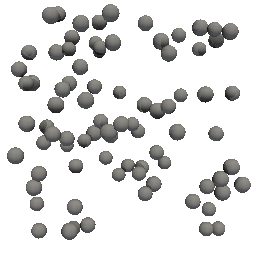
\includegraphics[width=0.14\columnwidth]{s2_slice_3D} &
	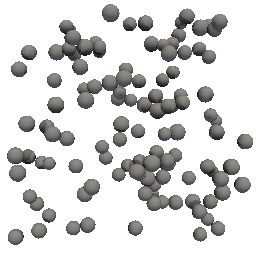
\includegraphics[width=0.14\columnwidth]{f2_slice_3D} &
	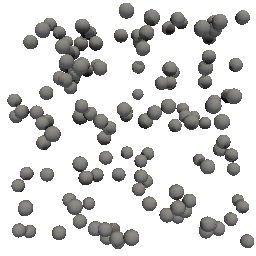
\includegraphics[width=0.14\columnwidth]{q6_slice_3D} &
	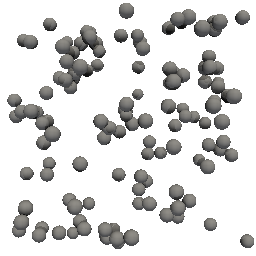
\includegraphics[width=0.14\columnwidth]{w6_slice_3D} &
	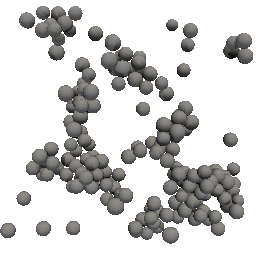
\includegraphics[width=0.14\columnwidth]{Q6_slice_3D} &
	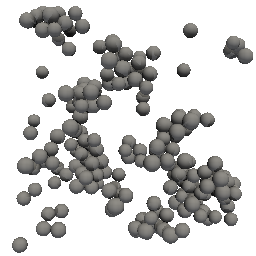
\includegraphics[width=0.14\columnwidth]{C_slice_3D}\\
	\end{tabu}
%\end{minipage}

\begin{minipage}[t][4\TPVertModule]{15\TPHorizModule}
\begin{tikzpicture}
	\pgfplotsset{fitc/.style={solid, no markers, forget plot, domain=0.05:5}}
	\begin{groupplot}[%
		group style={
			group name=Sq,
			group size=1 by 2,
			vertical sep=3em,
			},%
		width=3\TPHorizModule,
		height=8\baselineskip,%
		xlabel near ticks,
		xlabel shift=-0.5em,
		ylabel near ticks,
		xmode=log,
		ymode=log,%
		ytickten={-1,0,1}, yticklabels={0.1,~~1,10},
		ylabel absolute, every axis y label/.append style={anchor=base, yshift=1.5em},
		cycle list name=earthy,%
		legend style={at={(0.5,1.03)}, anchor=south},
		legend columns=10,
		]
		\nextgroupplot[%
			xlabel={$q\xi_{f_2}$}, ylabel={$S_{f_2}(q)/\chi_{f_2}$},
			xmin=0.05,xmax=2,%
			ymin=0.5, ymax=1.5, 
			]
			\addlegendimage{empty legend}
			%\addlegendimage{legend image code/.code={\node[right] {$P=$};}};
			%\addlegendentry{};
			\addplot+[only marks] table[x expr={0.076*\coordindex}, y expr={\thisrowno{0}/0.186}] {Sf2-std_P17.txt};
			\addplot+[only marks] table[x expr={0.0764*\coordindex}, y expr={\thisrowno{0}/0.176}] {Sf2-std_P19.txt};
			\addplot+[only marks] table[x expr={0.0742*\coordindex}, y expr={\thisrowno{0}/0.178}] {Sf2-std_P21.txt};
			\addplot+[only marks] table[x expr={0.0751*\coordindex}, y expr={\thisrowno{0}/0.178}] {Sf2-std_P23.txt};
			\addplot+[only marks] table[x expr={0.0731*\coordindex}, y expr={\thisrowno{0}/0.173}] {Sf2-std_P25.txt};
			\addplot+[black, fitc] {1/(1+x^2)};
			\legend{Pressures, $17$, $19$, $21$, $23$, $25$};
		
		\nextgroupplot[
			xlabel={$q\xi_{Q_6}$}, ylabel={$S_{Q_6}(q)/\chi_{Q_6}$},%
			xmin=0.1,xmax=10,%
			ymin=0.02, ymax=2,%
			]
			\addplot+[only marks] table[x expr={0.338*\coordindex}, y expr={\thisrowno{0}/0.937}] {SC-std_P17.txt};
			\addplot+[only marks] table[x expr={0.373*\coordindex}, y expr={\thisrowno{0}/1.22}] {SC-std_P19.txt};
			\addplot+[only marks] table[x expr={0.412*\coordindex}, y expr={\thisrowno{0}/1.32}] {SC-std_P21.txt};
			\addplot+[only marks] table[x expr={0.471*\coordindex}, y expr={\thisrowno{0}/1.61}] {SC-std_P23.txt};
			\addplot+[only marks] table[x expr={0.533*\coordindex}, y expr={\thisrowno{0}/2.23}] {SC-std_P25.txt};
			\addplot+[black, fitc] {1/(1+x^2)};
			\node[anchor=south west] at (rel axis cs:0,0) {$\displaystyle S_x(q\rightarrow 0) \approx \frac{\chi_x}{1+\xi_x^2 q^2}$};
			
	\end{groupplot}
	\begin{scope}
	\pgfplotsset{every axis/.append style={
		height=8\baselineskip,%
		width=3\TPHorizModule,
		cycle list name=exotic,
		xlabel={Pressure $\beta p\sigma^3$},
		ymin=0,
		xmin=8,
		xtick={9,13,...,25},
	}}
	\begin{axis}[%
		name=len,
		at={($(Sq c1r1.south east)+(\TPHorizModule,0)$)},
		ylabel={$\xi_x$},
		ymax=1.6,
		legend style={at={(1,1.03)}, anchor=south east},
		legend columns=10,
		]
	\pgfplotstableread{lengths.txt}\lengths
	 \foreach \y in {1, 2, ..., 6} {
          \addplot table[x index=0, y index=\y]{\lengths};
          \pgfplotstablegetcolumnnamebyindex{\y}\of{\lengths}\to{\colname}
          \addlegendentryexpanded{$\colname$}
          }
	\end{axis}
% 	\begin{axis}[%
% 		at={(len.below south west)},
% 		anchor=above north west,
% 		ylabel={$\chi_x$},
% 		ymax=2,
% 		]
% 	\pgfplotstableread{susceptibilities.txt}\sus
% 	 \foreach \y in {1, 2, ..., 6} {
%           \addplot table[x index=0, y index=\y]{\sus};
%           \pgfplotstablegetcolumnnamebyindex{\y}\of{\sus}\to{\colname}
%           }
% 	\end{axis}
	\end{scope}
	\begin{axis}[%
		at={($(Sq c1r2.south east)+(\TPHorizModule,0)$)},
		height=8\baselineskip,
		width=3\TPHorizModule,
		xlabel={Polydispersity $\Delta$ (\%)},
		ylabel={$\xi_x$},
		xmin=6, xmax=16, ymin=0,
		xtick={7,9,...,15},
		]
		\addplot+[black, mark=diamond] table[y index=2]{f2-std_P23.chixi} node[right] {$f_2$};
		\addplot+[Accent2, mark options={fill=Accent2}] table[y index=2]{w6-std_P23.chixi} node[right] {$w_6$};
		\addplot+[Accent1, mark options={fill=Accent1}] table[y index=2]{Q6-std_P23.chixi} node[right] {$Q_6$};
		%\legend{$f_2$,$w_6$,$Q_6$};
	\end{axis}
	\node[above right=0 of Sq c1r1.outer north west, inner xsep=0] (SqHead){\Subhead{Structure factors}};
	\node[anchor=base west, inner xsep=0] at (SqHead.base -| len.outer west){\Subhead{Correlation lengths}};
	\end{tikzpicture}
\end{minipage}
%\hfill
%\begin{minipage}[b][21.5\TPVertModule]{3\TPHorizModule}
%\begin{shaded*}
%	\Norulehead{Take home}
%	\Subhead{Over acidification}
%	\begin{itemize}
%		\item protein aggregates swell
%		\item power-law rheology, decreasing exponent
%		\item dissipation becomes glassy
%	\end{itemize}
%	\Subhead{Creep response}
%	\begin{itemize}
%		\item Andrade creep
%		\item finite time singularity
%		\item erratic transition
%	\end{itemize}
%	\Subhead{Fracture time prediction}
%	\begin{itemize}
%		\item composition influence limited to $G^\prime$
%		\item geometry factors as a nucleation rate
%	\end{itemize}
%\end{shaded*}
%
%
%	\vfill
%	\Head{Microscopy}
%	Final state without over-acidification\\
%	
%	\tikzsetnextfilename{structure_finale}
%	\input{fig_poster_palavas/structure_finale.pgf}
%	
%	\vfill
%	\Head{Monkman-Grant}
%	Predict failure from the minimum
%	
%	\tikzsetnextfilename{MonkmanGrant}
%	\input{fig_poster_palavas/MonkmanGrant.pgf}
%	Height-dependent near isoelectric\\
%	Upper bound for over-acidified
%	
%	
%	\vfill
%	\Head{Wavelength}
%	\tikzsetnextfilename{lambda}
%	\input{fig_poster_palavas/lambda.pgf}
%	Compatible with nucleation rate
%	
%\end{minipage}
%
%\vfill
%\small{\texttt{The research leading to these results has received funding from the European Research Council under the European Union's Seventh Framework Programme (FP7/2007-2013) / ERC grant agreement n°~258803.}}
%
%





\end{document}